\begin{frame}
  \titlepage
\end{frame}

\begin{frame}{Problem and objective}
  \begin{itemize}
    \item Life expectancy is a key indicator of a country's health and development.
    \item \textbf{Question:} which factors matter most, and how accurately can we predict it?
  \end{itemize}
  \vspace{0.5cm}
  \centering
  \begin{tikzpicture}[node distance=0.55cm, every node/.style={draw=aupp,fill=aupp!10,rounded corners=3pt,minimum width=2.6cm,minimum height=1.1cm,align=center,font=\small}]
    \node (a) {Clean\\{\footnotesize missing, invalid}};
    \node[right=of a] (b) {Explore\\{\footnotesize EDA, correlations}};
    \node[right=of b] (c) {Model\\{\footnotesize 4 models + baseline}};
    \node[right=of c] (d) {Interpret\\{\footnotesize drivers, errors}};
    \draw[-{Stealth},thick,aupp] (a)--(b); \draw[-{Stealth},thick,aupp] (b)--(c); \draw[-{Stealth},thick,aupp] (c)--(d);
  \end{tikzpicture}
\end{frame}
\note{Life expectancy summarizes health and development. We asked which factors matter most and how well we can predict it, following four steps: clean, explore, model, interpret.}

\begin{frame}{Dataset: Life Expectancy (WHO), Kaggle}
  \centering
  \stat{193}{countries} \hspace{0.3cm} \stat{2000--2015}{years} \hspace{0.3cm} \stat{2,938}{rows} \hspace{0.3cm} \stat{22}{variables}
  \vspace{0.4cm}
  \begin{columns}[T]
    \column{0.5\textwidth}
    \begin{itemize}
      \item \textbf{Target:} life expectancy (years)
      \item \textbf{Quantitative:} 18 predictors + year (e.g.\ adult mortality, GDP, schooling)
      \item \textbf{Qualitative:} country, status (Developed / Developing)
    \end{itemize}
    \column{0.5\textwidth}
    \begin{itemize}
      \item \textbf{Task:} supervised regression
      \item \textbf{After cleaning:} 2,928 rows, 183 countries, 24 columns
      \item \textbf{Issues:} missing values, implausible values, skewed features
    \end{itemize}
  \end{columns}
\end{frame}
\note{The data come from WHO via Kaggle. One row is one country in one year. Ten rows had no target value and were dropped, which removed ten countries.}

\begin{frame}{Data cleaning: missing and invalid values}
  \begin{columns}[T]
    \column{0.55\textwidth}
    \textbf{\color{aupp}Missing values} (14 of 22 columns)
    \begin{itemize}\small
      \item Population 22\%, hepatitis B 19\%, GDP 15\%
      \item Whole countries missing: population (48), GDP (30)
      \item Hepatitis B gaps: 98 rows (2000) $\to$ 9 (2015), so MAR
      \item Imputed: country median, then status median
    \end{itemize}
    \textbf{\color{aupp}Invalid values} (set to missing, then imputed)
    \begin{itemize}\small
      \item BMI outside 10--60: 629 rows; zero schooling: 26; zero income composition: 130
      \item Zero deaths with population $>$ 1M: 174 and 151
    \end{itemize}
    \column{0.45\textwidth}
    \centering
    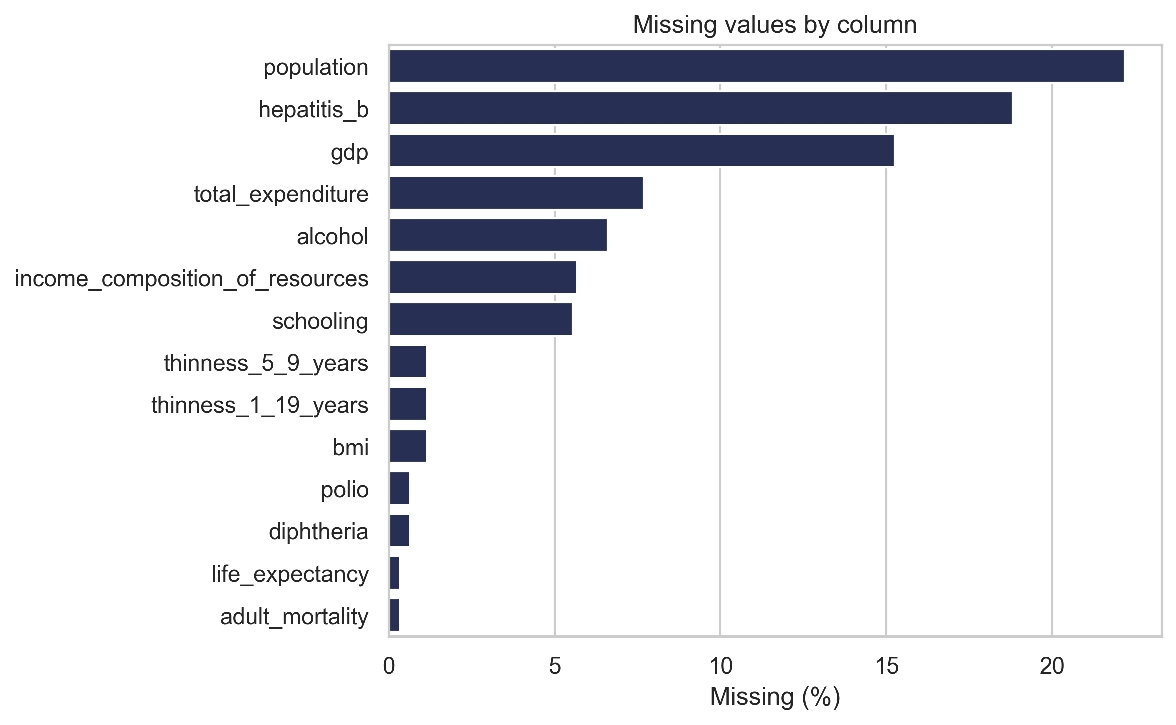
\includegraphics[width=\textwidth]{figs/missing_values_bar.pdf}
  \end{columns}
\end{frame}
\note{Missingness is not random: many countries are absent for every year, so we used the country median where possible and the status median otherwise. Impossible values such as BMI of 1 or 87 were set to missing and imputed. BMI stays a weak variable.}

\begin{frame}{Outliers and skewness}
  \begin{columns}[T]
    \column{0.52\textwidth}
    \begin{itemize}
      \item IQR flags 15--19\% of rows for measles, HIV/AIDS, GDP, population
      \item These are genuine (large or severely affected countries) $\Rightarrow$ \textbf{kept}
      \item Instead, \textbf{$\log(1+x)$} on 9 skewed features
    \end{itemize}
    \column{0.48\textwidth}
    \centering\small
    \begin{tabular}{lrr}\toprule
      \textbf{Feature} & \textbf{Before} & \textbf{After}\\\midrule
      population & 17.94 & $-0.37$\\
      infant deaths & 9.77 & 0.70\\
      measles & 9.43 & 0.55\\
      HIV/AIDS & 5.39 & 2.12\\
      GDP & 3.46 & $-0.10$\\\bottomrule
    \end{tabular}\\[2pt]{\footnotesize Skewness before and after transform}
  \end{columns}
\end{frame}
\note{Removing these points would delete real information, so we kept them and reduced the skew with a log transform. Immunization variables are left-skewed, so they were not transformed.}

\begin{frame}{EDA: the development gap}
  \centering
  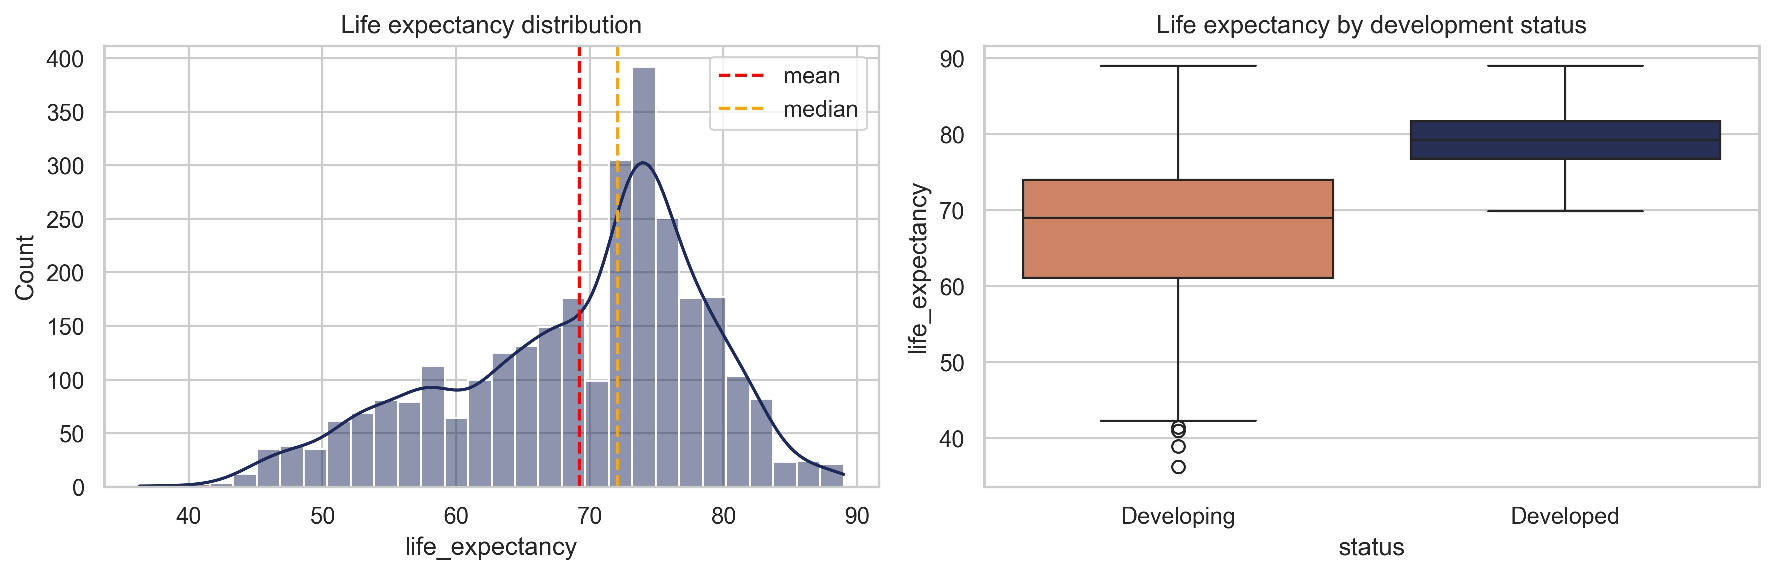
\includegraphics[width=0.92\textwidth]{figs/target_distribution.pdf}
  \begin{itemize}\small
    \item Mean 69.2 years, SD 9.5, left-skewed: a long tail of low values
    \item \textbf{Developed 79.2 vs.\ Developing 67.1} years (Welch $t=47.9$, $p<0.001$)
    \item Gap narrowed from 12.2 (2000) to 11.0 years (2015); Developing +5.1, Developed +3.9
  \end{itemize}
\end{frame}
\note{Developed countries live about twelve years longer. Both groups improved, and developing countries improved faster, so the gap is narrowing.}

\begin{frame}{EDA: what correlates with life expectancy?}
  \centering
  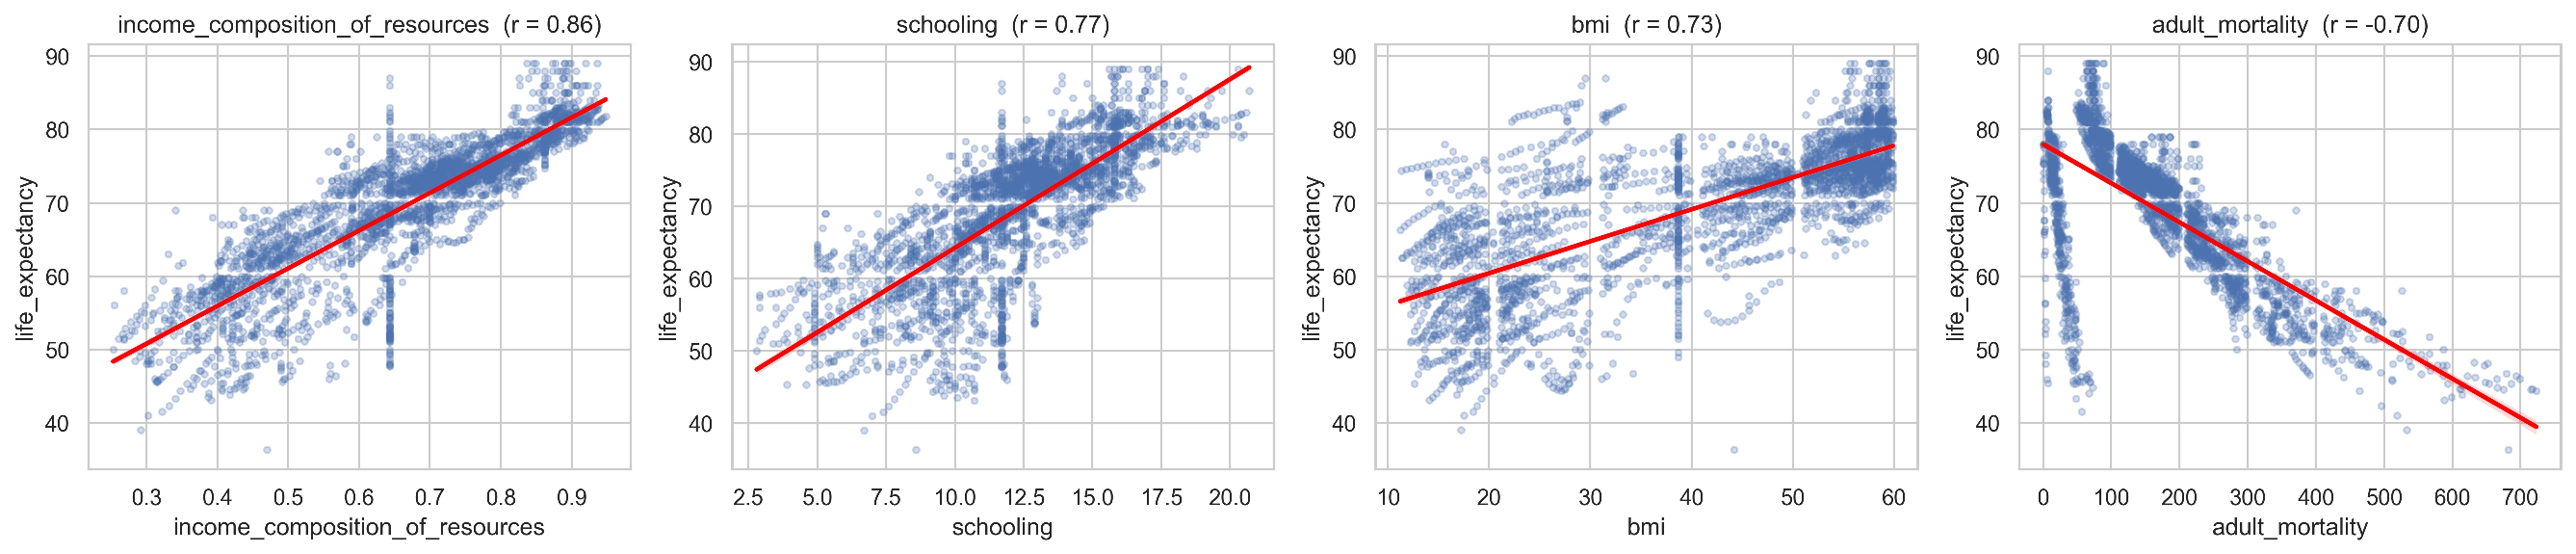
\includegraphics[width=\textwidth]{figs/scatter_top4.pdf}
  \begin{itemize}\small
    \item Strongest: income composition ($r=0.86$), schooling (0.77), BMI (0.73), adult mortality ($-0.70$)
    \item Spearman $\gg$ Pearson for infant deaths ($-0.60$ vs $-0.20$), HIV/AIDS ($-0.75$ vs $-0.56$), GDP $\Rightarrow$ \textbf{non-linear}
    \item Income composition and schooling overlap ($r=0.92$, VIF 12.6)
  \end{itemize}
\end{frame}
\note{The top four relationships are clear, but several variables relate to the target in a monotonic, non-linear way, which hints that tree models may do better than a straight line.}

\begin{frame}{EDA hypotheses}
  \centering\small
  \renewcommand{\arraystretch}{1.5}
  \begin{tabularx}{\textwidth}{lXc}\toprule
    \textbf{Hypothesis} & \textbf{Evidence} & \textbf{Result}\\\midrule
    $H_1$: more schooling, longer life & $r=0.77$ (Spearman 0.81) & {\color{teal}$\checkmark$}\\
    $H_2$: Developed $>$ Developing & +12.1 years; $t=47.9$; ANOVA by GDP tier $F=691$ & {\color{teal}$\checkmark$}\\
    $H_3$: adult mortality lowers life expectancy & $r=-0.70$; HIV/AIDS also strongly negative ($-0.56$) & {\color{teal}$\checkmark$}\\\bottomrule
  \end{tabularx}
\end{frame}
\note{All three hypotheses are supported by the exploratory analysis. Later we check whether the models agree.}

\begin{frame}{Modeling pipeline}
  \centering
  \begin{tikzpicture}[node distance=0.45cm, every node/.style={draw=aupp,fill=aupp!10,rounded corners=3pt,minimum width=2.8cm,minimum height=1.3cm,align=center,font=\small}]
    \node (a) {Split \textbf{by country}\\{\footnotesize 80/20: 146 / 37 countries}};
    \node[right=of a] (b) {Scale\\{\footnotesize fit on train only}};
    \node[right=of b] (c) {Train 4 models\\{\footnotesize + mean baseline}};
    \node[right=of c] (d) {Evaluate\\{\footnotesize 5-fold grouped CV + test}};
    \draw[-{Stealth},thick,aupp] (a)--(b); \draw[-{Stealth},thick,aupp] (b)--(c); \draw[-{Stealth},thick,aupp] (c)--(d);
  \end{tikzpicture}
  \vspace{0.3cm}
  \begin{itemize}\small
    \item 18 features; two near-duplicates dropped (under-five deaths, thinness 5--9)
    \item Linear, Ridge ($\alpha=10$ by grouped CV), Random Forest (300 trees), Gradient Boosting
    \item Splitting by country prevents the same country appearing in train and test
  \end{itemize}
\end{frame}
\note{We split by country, not by row, because rows from the same country across years are very similar and would leak information. Ridge alpha was tuned by cross-validation; the tree models used default settings.}

\begin{frame}{Results: model comparison}
  \begin{columns}[T]
    \column{0.6\textwidth}
    \centering\footnotesize
    \begin{tabular}{lcccc}\toprule
      \textbf{Model} & \textbf{CV RMSE} & \textbf{Test RMSE} & \textbf{MAE} & \textbf{$R^2$}\\\midrule
      Baseline (mean) & -- & 9.95 & 7.98 & $-0.06$\\
      Linear & 3.65 & 3.24 & 2.51 & 0.888\\
      Ridge & 3.65 & 3.24 & 2.50 & 0.888\\
      Random Forest & 3.00 & 2.65 & 1.93 & 0.925\\
      Gradient Boosting & 3.01 & \textbf{2.59} & 1.95 & \textbf{0.928}\\\bottomrule
    \end{tabular}
    \column{0.4\textwidth}
    \begin{itemize}\small
      \item Best: \textbf{Gradient Boosting}, error cut by 74\% vs.\ baseline
      \item Tree ensembles beat linear models by about 20\%
      \item RF and GB are nearly tied
    \end{itemize}
  \end{columns}
  \vspace{0.2cm}
  \centering
  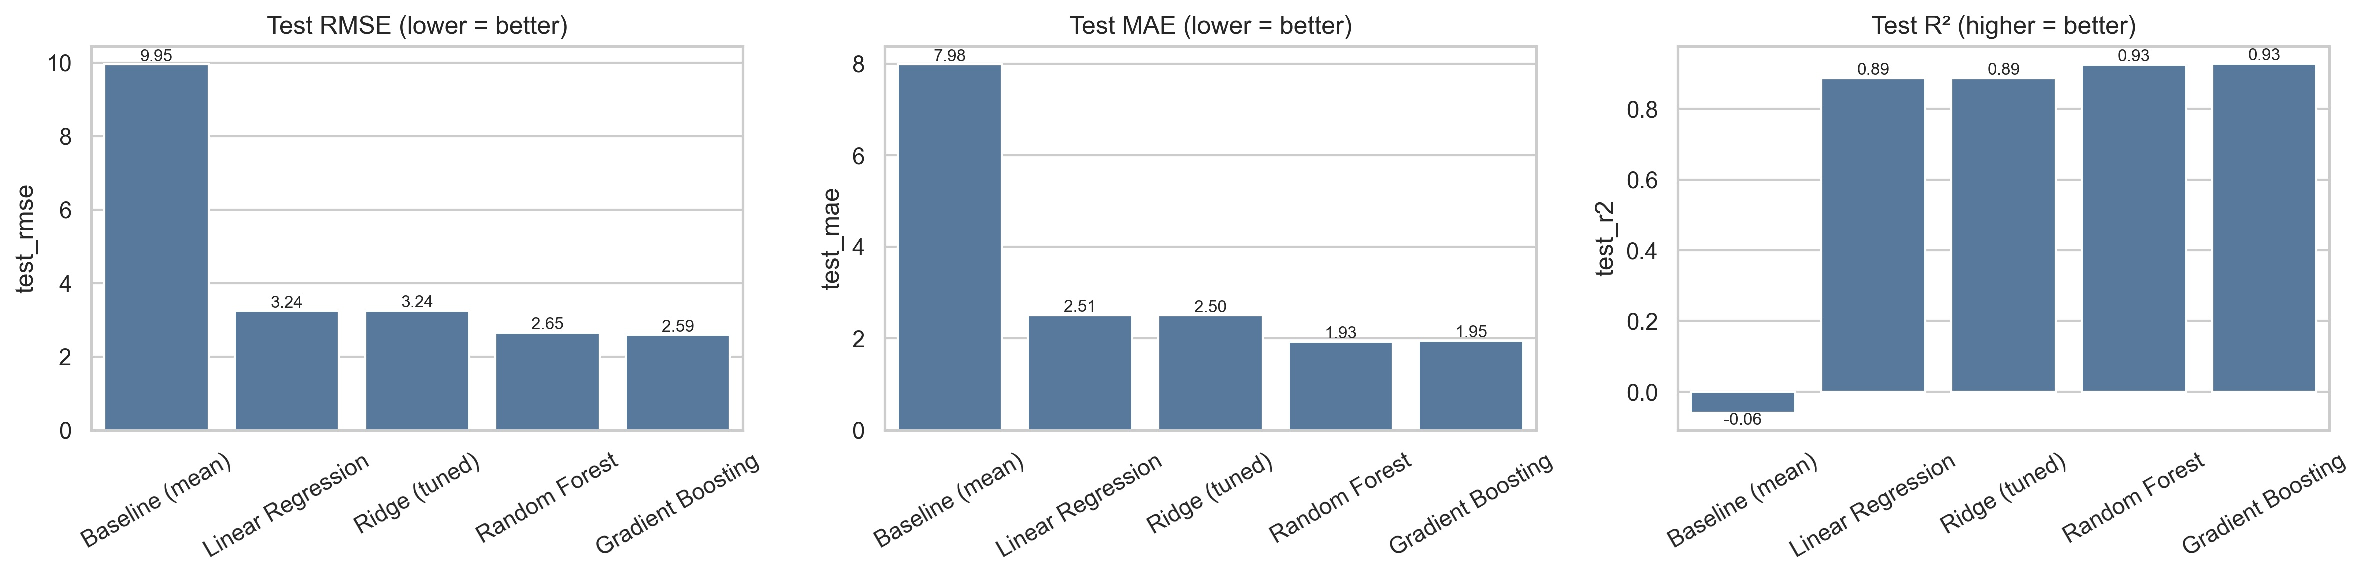
\includegraphics[width=0.85\textwidth]{figs/model_comparison.pdf}
\end{frame}
\note{All models beat the baseline. Gradient Boosting has the lowest test error, but Random Forest is within 0.06 years and has a slightly lower cross-validation error, so we do not claim a clear winner. Test error is lower than CV error because the test set has only 37 countries.}

\begin{frame}{Predicted vs.\ actual (Gradient Boosting)}
  \centering
  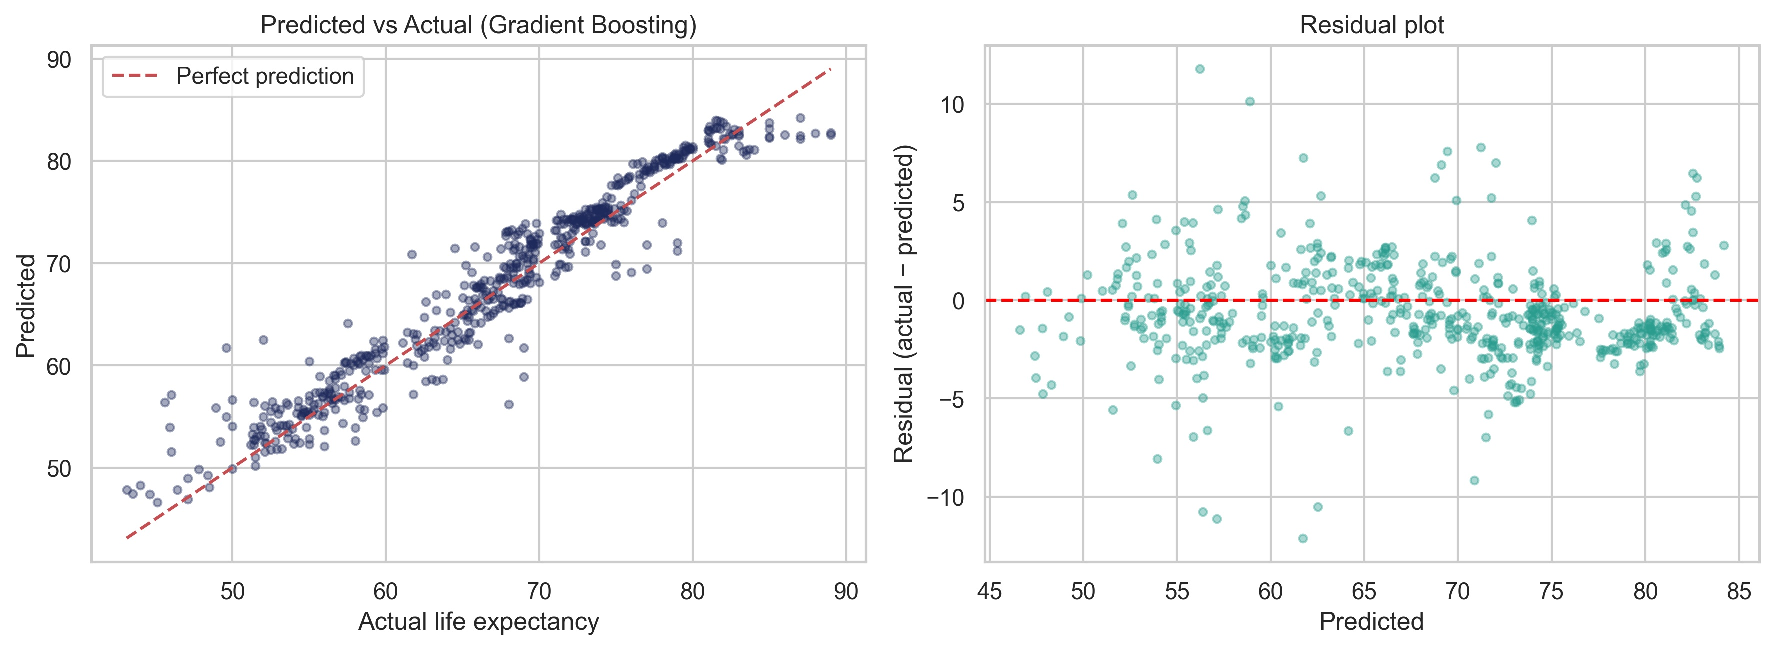
\includegraphics[width=0.9\textwidth]{figs/pred_vs_actual_residuals.pdf}
  \begin{itemize}\small
    \item Typical error about \textbf{2 years} (MAE 1.95) against an SD of 9.5
    \item Most residuals within $\pm5$ years; mean residual $-0.7$ (slight over-prediction)
    \item Predictions flatten at the extremes (below 50 and above 82 years)
  \end{itemize}
\end{frame}
\note{Predictions follow the diagonal closely. The model is least accurate for the very lowest and highest life expectancies, where there are few countries.}

\begin{frame}{What drives life expectancy?}
  \begin{columns}[T]
    \column{0.49\textwidth}
    \centering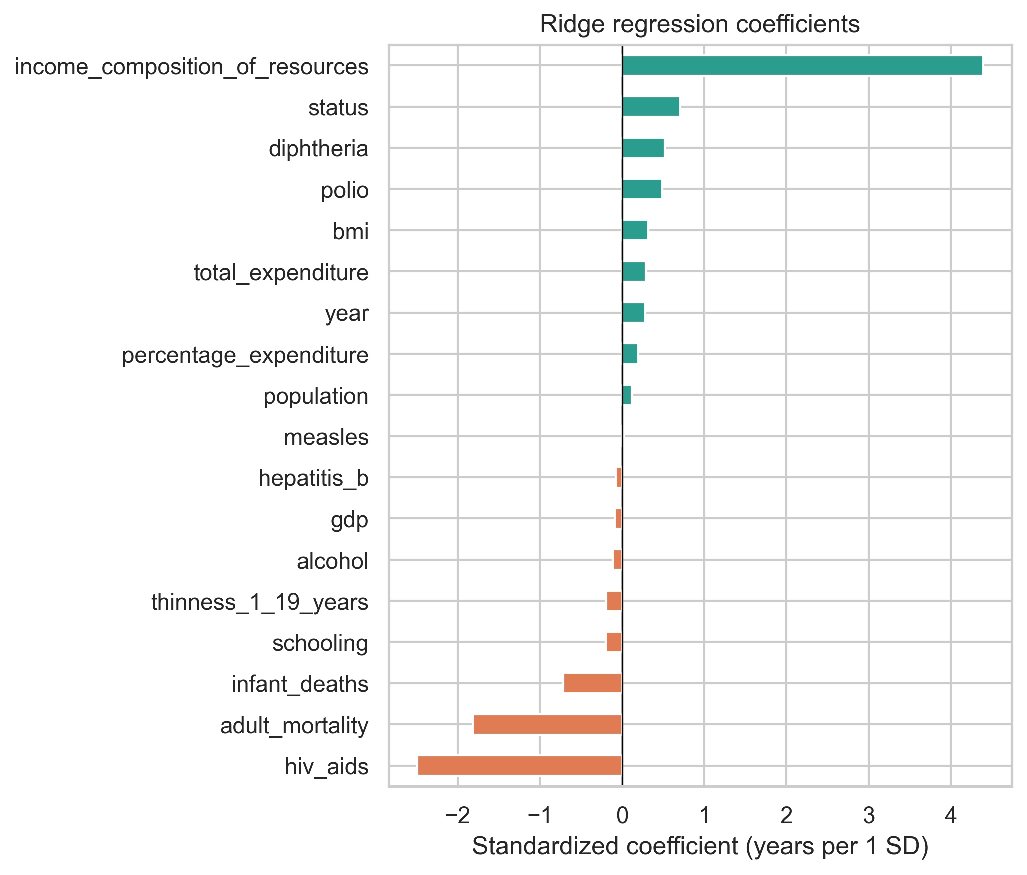
\includegraphics[height=5.3cm]{figs/ridge_coefficients.pdf}
    \column{0.49\textwidth}
    \centering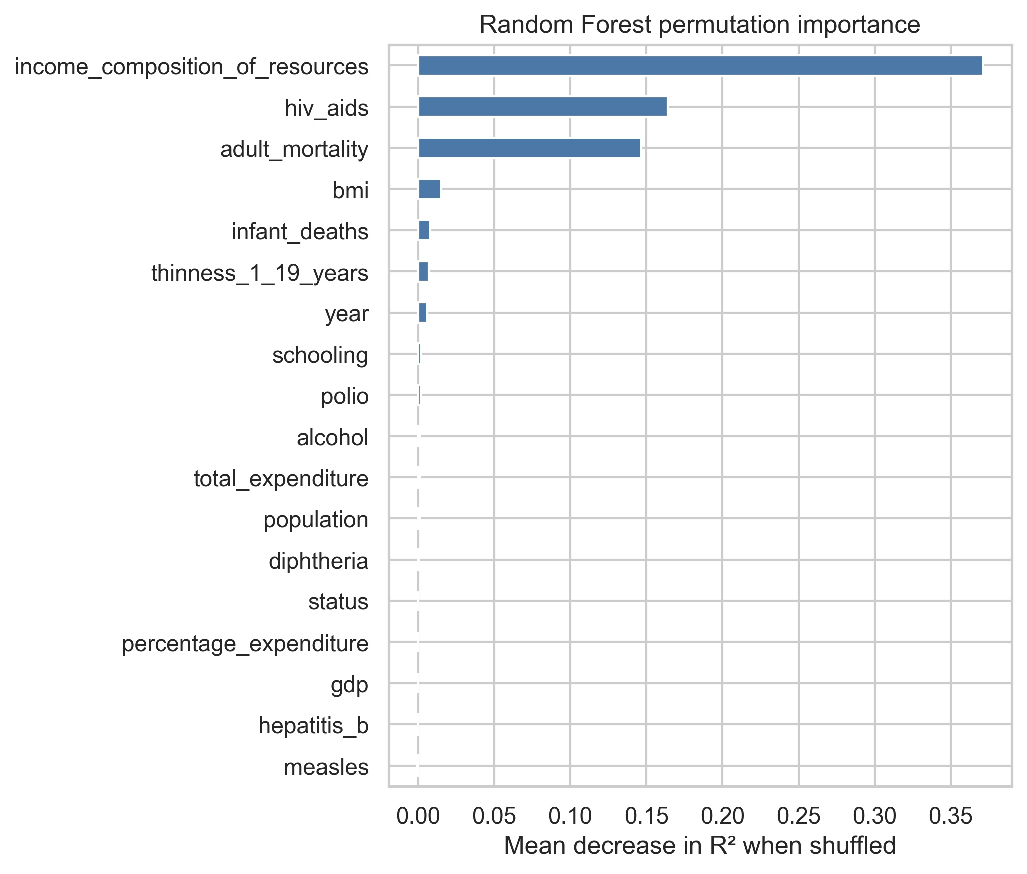
\includegraphics[height=5.3cm]{figs/rf_permutation_importance.pdf}
  \end{columns}
  \vspace{0.1cm}
  \begin{itemize}\footnotesize
    \item Both models agree on the top 3: \textbf{income composition}, \textbf{HIV/AIDS}, \textbf{adult mortality}
    \item Schooling's coefficient is slightly negative because it overlaps with income composition ($r=0.92$)
  \end{itemize}
\end{frame}
\note{A linear model and a non-linear model rank the same three drivers first. The negative schooling coefficient is a collinearity effect, not evidence that education is harmful; its relationship with life expectancy is strongly positive on its own.}

\begin{frame}{Conclusion and implications}
  \begin{enumerate}
    \item Life expectancy is predictable: test RMSE \textbf{2.59 years}, $R^2=0.93$
    \item Non-linear models fit better than linear ones
    \item Main drivers: income composition, HIV/AIDS, adult mortality
    \item Developed--Developing gap: 12 years, slowly narrowing
  \end{enumerate}
  \vspace{0.2cm}
  \begin{block}{Implications}
    \small Prioritize HIV/AIDS and adult mortality reduction and broad development; use the model to
    estimate life expectancy where data are incomplete.
  \end{block}
\end{frame}
\note{The model predicts within about two years. For policy, the biggest levers are HIV/AIDS, adult mortality and the overall development level.}

\begin{frame}{Limitations and future work}
  \begin{columns}[T]
    \column{0.5\textwidth}
    \textbf{\color{aupp}Limitations}
    \begin{itemize}\small
      \item Imputation: whole countries missing population / GDP
      \item BMI unreliable (629 invalid rows)
      \item Country-level data; correlation $\neq$ causation
      \item Single split, 37 test countries; trees untuned
      \item Income composition may overlap with the target
    \end{itemize}
    \column{0.5\textwidth}
    \textbf{\color{aupp}Future work}
    \begin{itemize}\small
      \item Tune RF / GB; repeat splits for confidence intervals
      \item Panel or mixed-effects models over time
      \item Better external data; years after 2015
      \item Sensitivity: drop BMI, schooling or income composition
    \end{itemize}
  \end{columns}
\end{frame}
\note{We are explicit about the main weaknesses: imputed data for some countries, a weak BMI variable, country-level averages, and a single small test set.}
